\section{eo\-Init\-Variable\-Length$<$ EOT $>$ Class Template Reference}
\label{classeo_init_variable_length}\index{eoInitVariableLength@{eoInitVariableLength}}
Initializer for variable length representations with a single type.  


{\tt \#include $<$eo\-Init.h$>$}

Inheritance diagram for eo\-Init\-Variable\-Length$<$ EOT $>$::\begin{figure}[H]
\begin{center}
\leavevmode
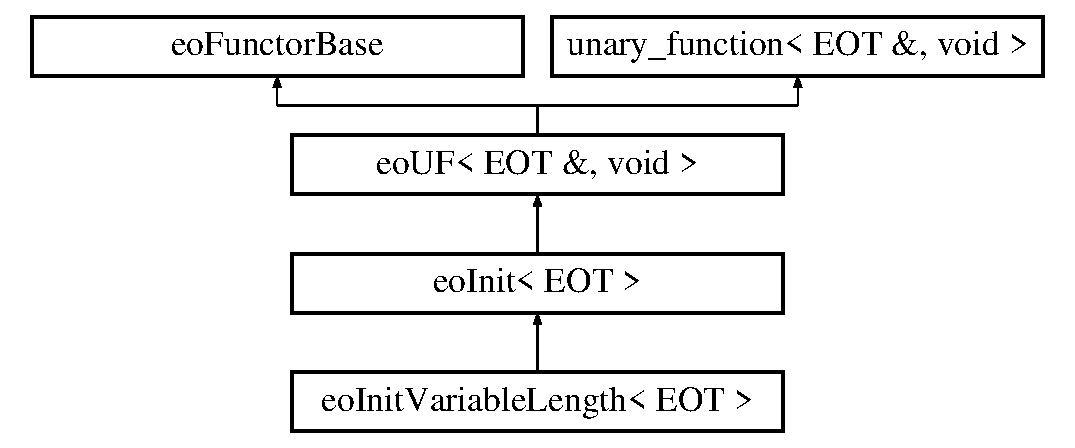
\includegraphics[height=4cm]{classeo_init_variable_length}
\end{center}
\end{figure}
\subsection*{Public Types}
\begin{CompactItemize}
\item 
typedef EOT::Atom\-Type {\bf Atom\-Type}\label{classeo_init_variable_length_w0}

\end{CompactItemize}
\subsection*{Public Member Functions}
\begin{CompactItemize}
\item 
{\bf eo\-Init\-Variable\-Length} (unsigned \_\-min\-Size, unsigned \_\-max\-Size, {\bf eo\-Init}$<$ Atom\-Type $>$ \&\_\-init)\label{classeo_init_variable_length_a0}

\begin{CompactList}\small\item\em Ctor from an {\bf eo\-Init}{\rm (p.\,\pageref{classeo_init})}. \item\end{CompactList}\item 
virtual void {\bf operator()} ({\bf EOT} \&\_\-chrom)\label{classeo_init_variable_length_a1}

\begin{CompactList}\small\item\em The pure virtual function that needs to be implemented by the subclass. \item\end{CompactList}\item 
{\bf eo\-Init}$<$ Atom\-Type $>$ \& {\bf atom\-Init} ()\label{classeo_init_variable_length_a2}

\end{CompactItemize}
\subsection*{Private Attributes}
\begin{CompactItemize}
\item 
unsigned {\bf offset}\label{classeo_init_variable_length_r0}

\item 
unsigned {\bf extent}\label{classeo_init_variable_length_r1}

\item 
{\bf eo\-Init}$<$ Atom\-Type $>$ \& {\bf init}\label{classeo_init_variable_length_r2}

\end{CompactItemize}


\subsection{Detailed Description}
\subsubsection*{template$<$class EOT$>$ class eo\-Init\-Variable\-Length$<$ EOT $>$}

Initializer for variable length representations with a single type. 



Definition at line 107 of file eo\-Init.h.

The documentation for this class was generated from the following file:\begin{CompactItemize}
\item 
eo\-Init.h\end{CompactItemize}
